\section{Turnstile Example}
\label{sec:example}

A turnstile is used to illustrate the construction of a system model under the developed semantics. 
%Starting from a statechart diagram and its corresponding XML textual representation, the Event-B verification tool can then be used to support both the model construction and verification. 
Figure~\ref{fig:turnstile} shows the statechart diagram for the turnstile. The system has two sub-components that manage the operations performed by the gate and card reader in the turnstile. These components are represented by the \emph{GATE} and \emph{CARD\_READER} parallel regions, respectively. 
\begin{figure}[!th]
\centering
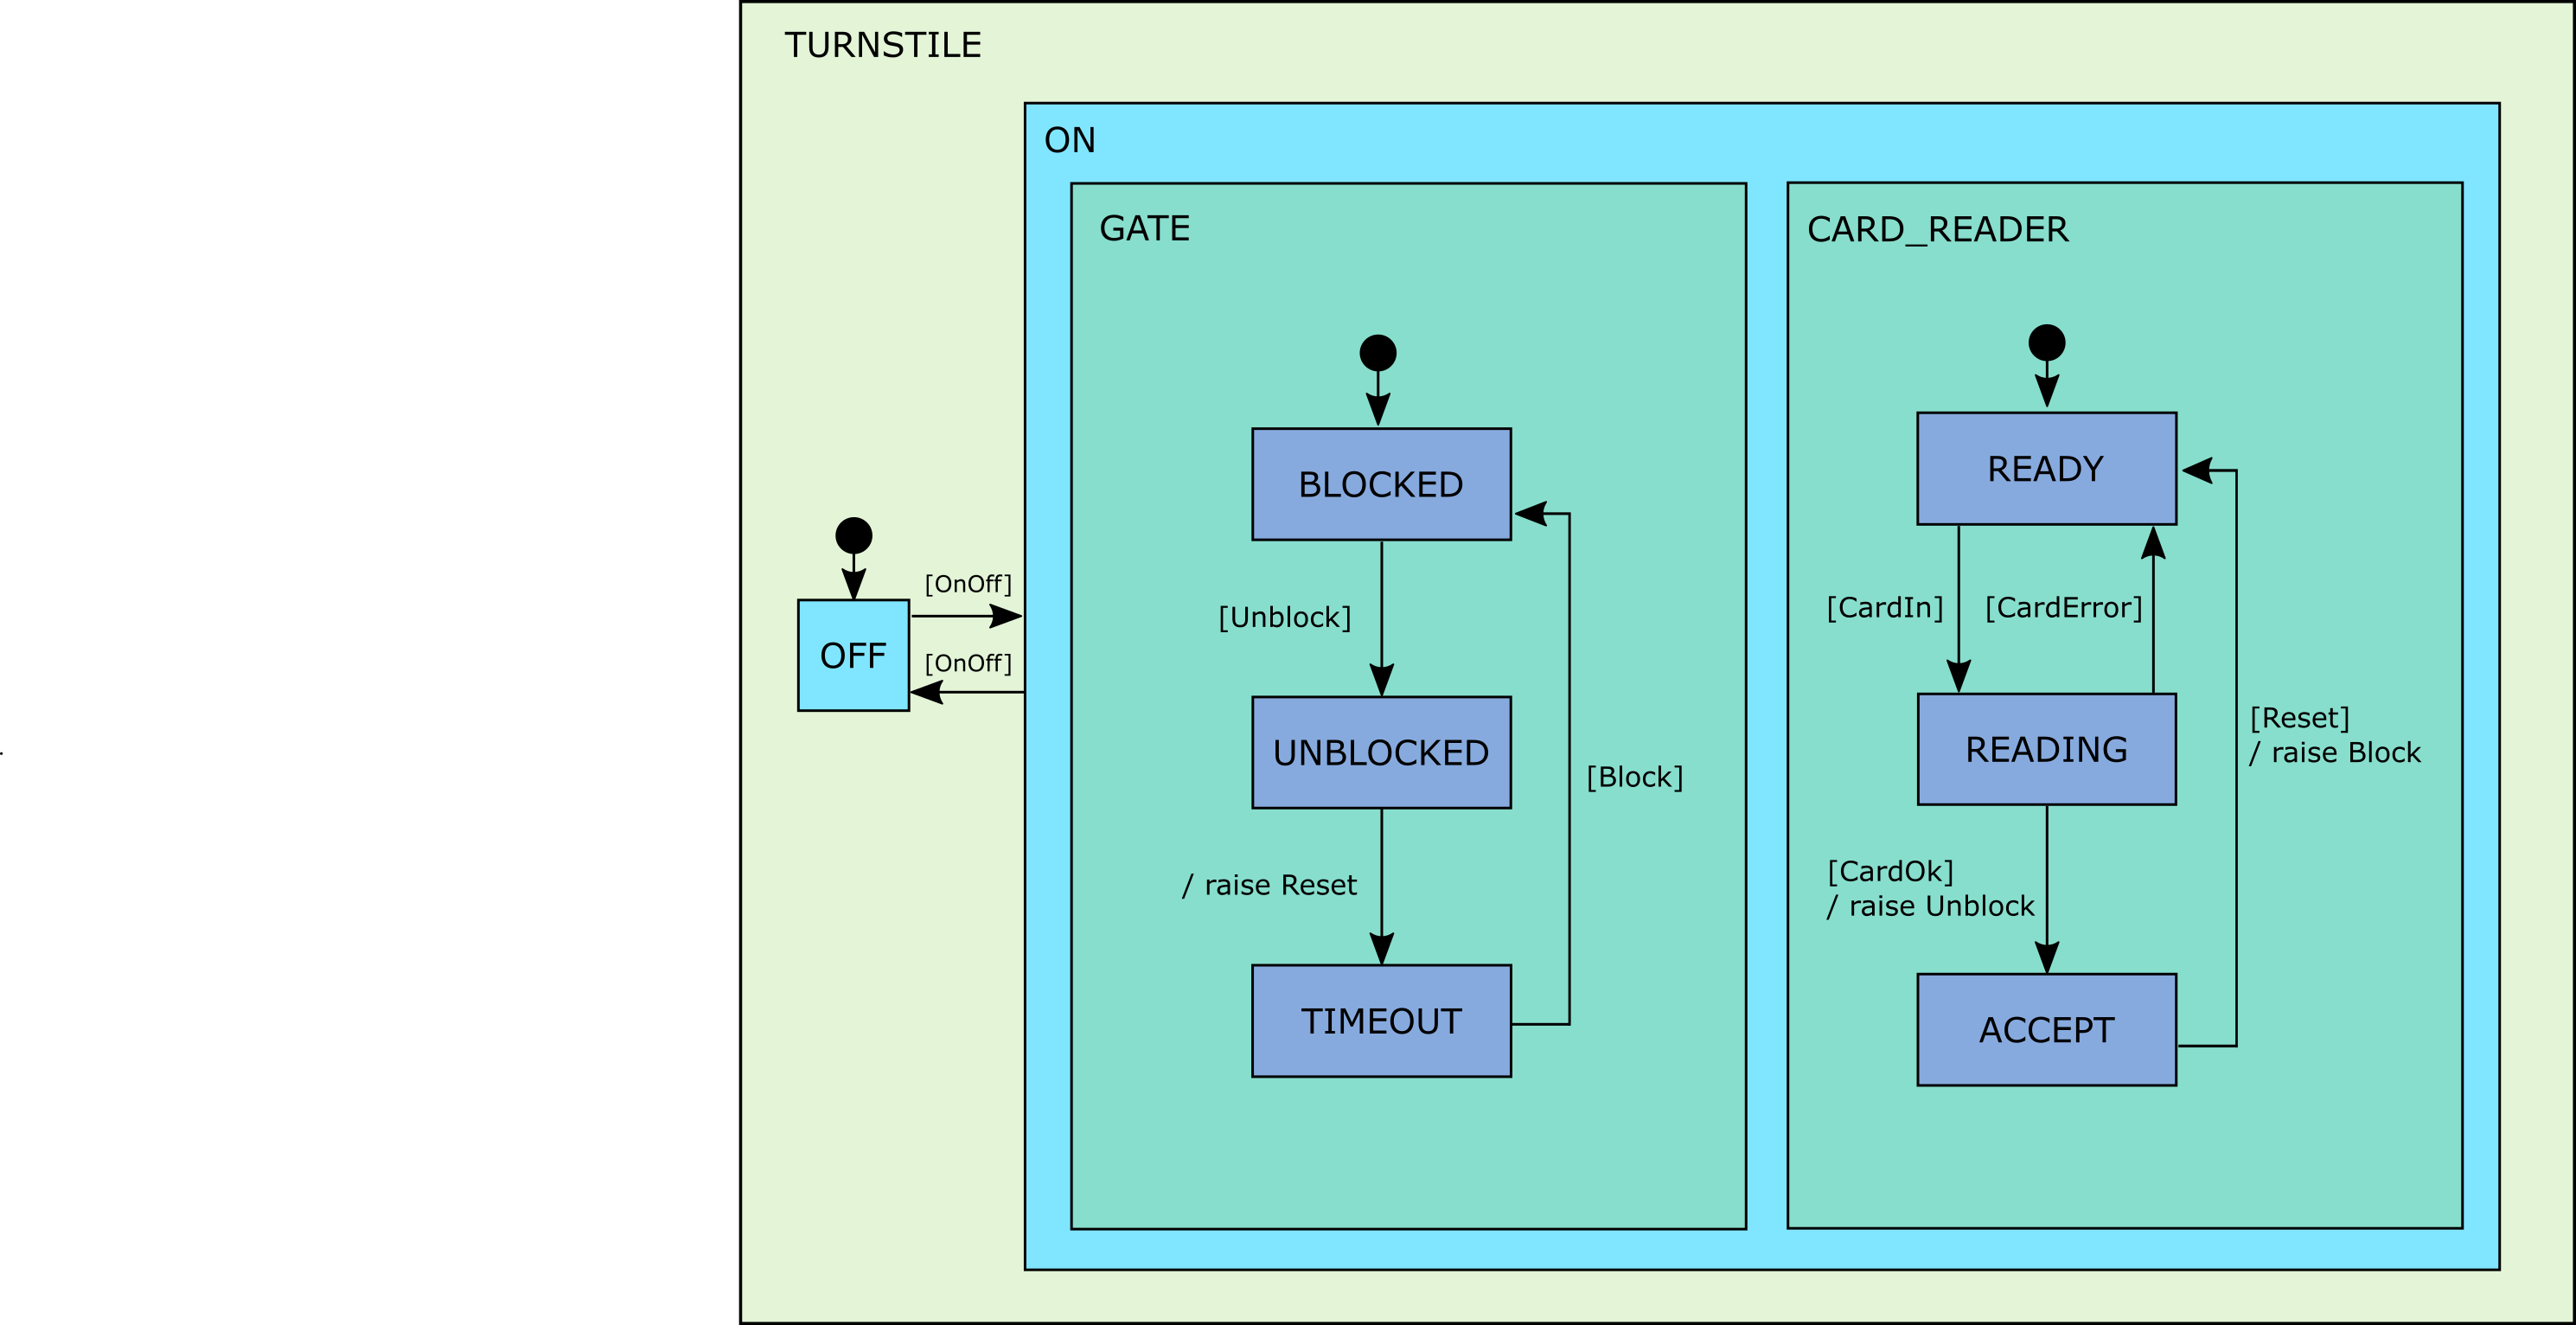
\includegraphics[trim={25cm 0 0 0}, width=0.7\textwidth]{figures/Turnstile.png}
\caption{Design model for a turnstile system}
\label{fig:turnstile}
\end{figure}

The model has two external triggers (\emph{OnOff}, and \emph{CardIn}), which are signals provided by the environment under which the system operates. In addition, there are internal triggers (\emph{CardOk}, \emph{Unblock}, \emph{Block}, and \emph{Reset}) that are raised by the components in the system. Transitions from source to target state are guarded by the specified conditions (i.e., [Unblock], \emph{Unblock} trigger is in the queue). Actions associated with a specific transition are expressed as 
|\raise Trigger|, which result in adding the trigger to the queue. In the current model some of the internal triggers are raised non-deterministically (e.g. \emph{CardOk}, \emph{CardError}), as the details of the actual mechanisms responsible for the generation of the signal are not fully specified. Even in the presence of this non-determinism the system must satisfy certain requirements. 
Refinement of the abstract model presented in Figure~\ref{fig:turnstile} can be used to incorporate implementation details. 
For example, a nested  statechart could be added to the \emph{READING} state to specify the process by which the aforementioned triggers are  raised. 
This manuscript focuses on formalizing the modeling language semantics for triggered statecharts of this form, and leaves the extensions required for refinement proofs to a future publication.  
%The following sections will describe in detailed each of the semantic models constructed to support a specification and formal analysis of this system using our modeling language.